\documentclass[12pt]{article}
\usepackage[english]{babel}
\usepackage[utf8x]{inputenc}
\usepackage{amsmath}
\usepackage{tikz}
\usetikzlibrary{arrows,automata}
\begin{document}

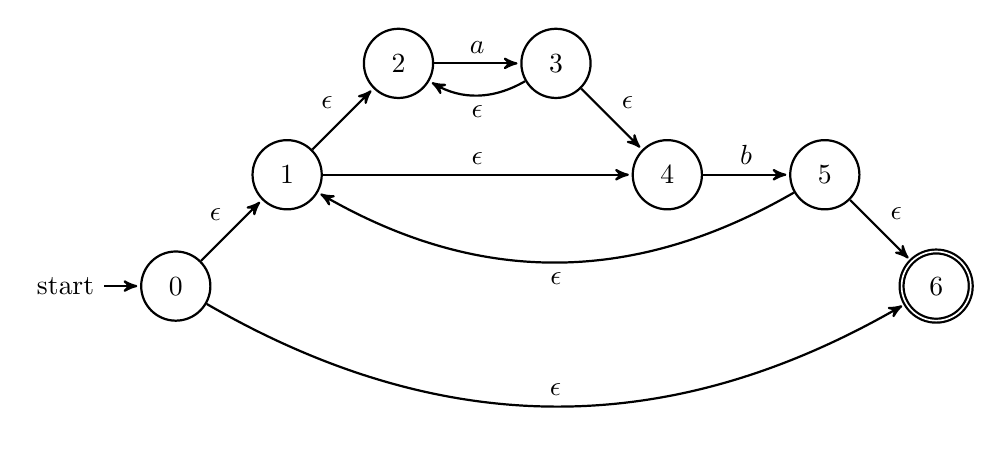
\begin{tikzpicture}[->,>=stealth',shorten >=1pt,auto,node distance=2cm,
    thick,base node/.style={circle,draw,minimum size=8pt}, real node/.style={double,circle,draw,minimum size=17pt}]

  \node[state]          (a){$2$};
  \node[state]  (start) [below left of=a]{$1$};
  \node[state,initial]  (zero) [below left of=start]{$0$};
  \node[state]          (b) [right of=a] {$3$};
  \node[state]          (c)  [below right of=b] {$4$};
  \node[state] (d)  [right of=c] {$5$};
  \node[state,accepting] (end)  [below right of=d] {$6$};
  \path (start) edge node {$\epsilon$} (a)
        (a) edge    node {$a$} (b)
        (start) edge node {$\epsilon$} (c)
        (b) edge [bend left] node {$\epsilon$} (a)
        (b) edge      node {$\epsilon$} (c)
        (c) edge node {$b$} (d) 
        (zero) edge node {$\epsilon$} (start)
        (d) edge node {$\epsilon{}$} (end)
        (zero) [bend right] edge node {$\epsilon$} (end)
        (d) [bend left] edge node {$\epsilon$} (start)
        ;
\end{tikzpicture}
\end{document}